\chapter{前言}

\linespread{1.5}\selectfont
\begin{multicols}{2}
物種或分類群(taxon)是生物多樣性保育上 所有人可以理解的階層(IUCN Red List Committee 2013)。
國際自然保育聯盟 (International Union for Conservation of Nature, IUCN)從成立開始,
就支持物種保育工作; 1950 年成立物種存續委 員會(Species Survival Commission),
並從 1963 年開始倡導紅皮書的概念(IUCN/UNEP et al. 1987)。
現在紅皮書已成為評估全球物種保育狀況與變化趨勢最重要的參考依據(Rodrigues et al. 2006 ; IUCN Red List Committee 2013),
另其類別(圖 \ref{fig1}) 及評估標準(criteria),乃至後續發布的 IUCN 紅皮書名錄地區及國家級評估標準應用指南,
亦成為許多國家評估其國境內受脅物種名錄的首要參考依據(Townsend et al. 2007 ; IUCN Standards and Petitions Subcommittee 2017)。
藉此標準化的評估方法,不僅有助於各國立法、執法與爭取社會支持;而依威脅程度所列出的清單,也是各種復育計畫、
棲地保護、研究、監測、資源分配與保育措施排列優先順序的重要參考工具 (Townsend et al. 2007)。\\

IUCN 紅皮書原是以全球做為評估範圍的,如果一個地區、國家或地方性的紅皮書的產生是依據 IUCN 系統,
那麼就必須無偏差地根據 IUCN 紅皮書類別及標準(IUCN Red List Categories and Criteria)進行評估(IUCN 2012b);
但由全球轉至地區(包括地區、國家及地方)進行評估時,對受威脅物種而言,自然會產生原生或外來種,
繁殖或非繁殖物種,或如先前曾經分布,但已局部滅絕的區域現象(IUCN 2012a)。
也就是說,由於空間尺度的關係,當全球的標準應用於分布不完全侷限於評估範圍的物種時,
評估流程與標準設定的閥值可能並不適當,因此必須有所有調整,
IUCN 從 1999 年開始對於紅皮書名錄地區及國家級評估標準應用指南提供調整建議(Gärdenfors 1999;IUCN 2012a)。
本報告採用的評估標準與類別係依據 IUCN 紅皮書名錄類別與標準 3.1 版(IUCN 2012b),
並以地區及國家階層的應用指引: 4.0 版(IUCN 2012a)進行調整。\\

全球植物紅皮書現有的主要清單(Oldfield et al. 1998; Walter and Gillett 1998),
由於不是以現今的標準進行評估,因此絕大部分不能使用,僅有蘇鐵類及松柏類植物可以使用;
少數分類群雖使用修改過後的標準進行全球的物種評估
(Cicuzza et al. 2007;Gibbs and Chen 2009;Gibbs et al. 2011;Oldfield and Eastwood 2007),
但這些書中亦指出內中有不少的分類爭議及資訊不足之處,尤以臺灣的物種多是以 Flora of China 為基礎進行評估,
分類及評估標準爭議更是明顯,更需要從區域進行標準化的評估,保育類別的資訊方能更為精準。 \\

臺灣野生的維管束植物超過五千種,其中約有四分之ㄧ為特有種,豐富之植物種類實為國家重要的資源,
然近年來環境破壞日益加劇,頗多物種已面臨滅絕的危機,
特有生物研究保育中心與臺灣植物分類學會於 2008 至 2010 年合作,
使用 IUCN 紅皮書類別及標準進行臺灣地區野生維管束植物的物種存活受威脅程度評估---
「建構全國生物物種多樣性指標系統---植物紅皮書編纂及出版」,累計三年共完成 4,174 種之評估,
其中屬於受威脅(包括嚴重瀕臨絕滅、瀕臨絕滅及易受害)之物種共 908 種,
並出版「臺灣維管束植物紅皮書初評名錄」(王震哲等,2012)。然自該計畫結束後,
植物學者陸續發表之臺灣新種或新紀錄種達 300 種以上,
而許多原受評為受威脅物種者此期間亦新增諸多族群資訊與分類資料,需予以重新評估審定。
本報告蒐集及更新臺灣所有野生維管束植物的分布範圍、族群趨勢、數量與受脅原因等資訊,
依據 IUCN 類別與標準評估各植物物種的最新受威脅狀態。\\
\end{multicols}
\begin{figure}[!ht]
    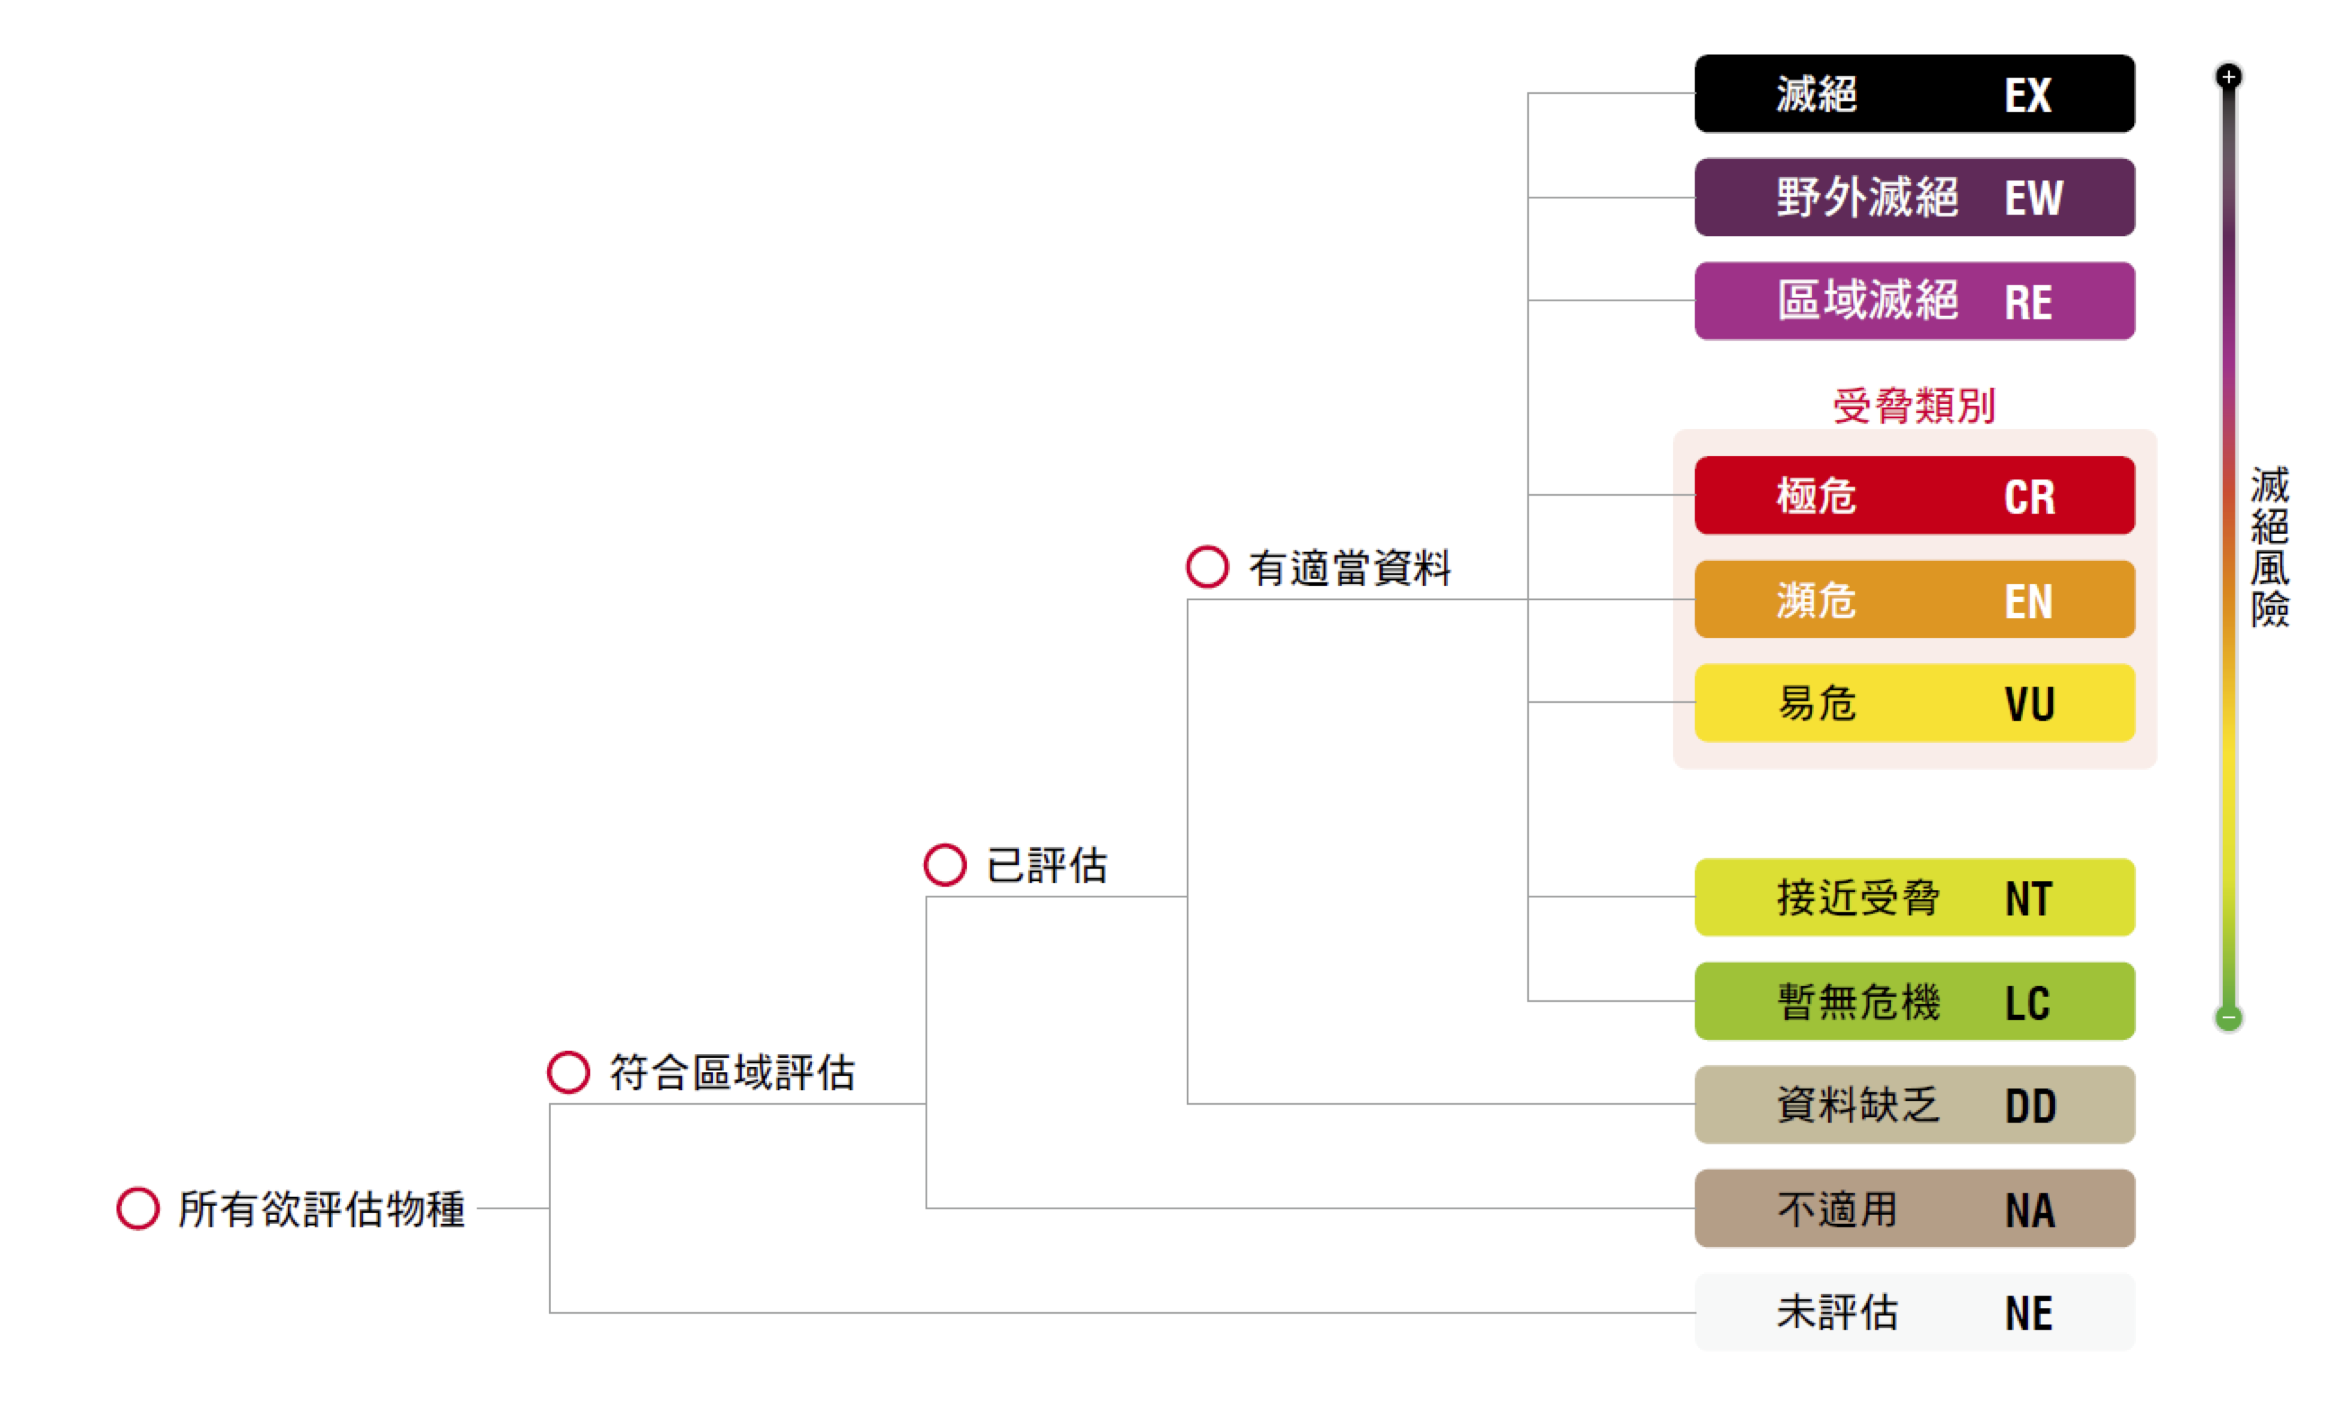
\includegraphics[width=\textwidth]{images/fig1.png}
    \caption{IUCN 國家或區域紅皮書類別} \label{fig1}
\end{figure}

%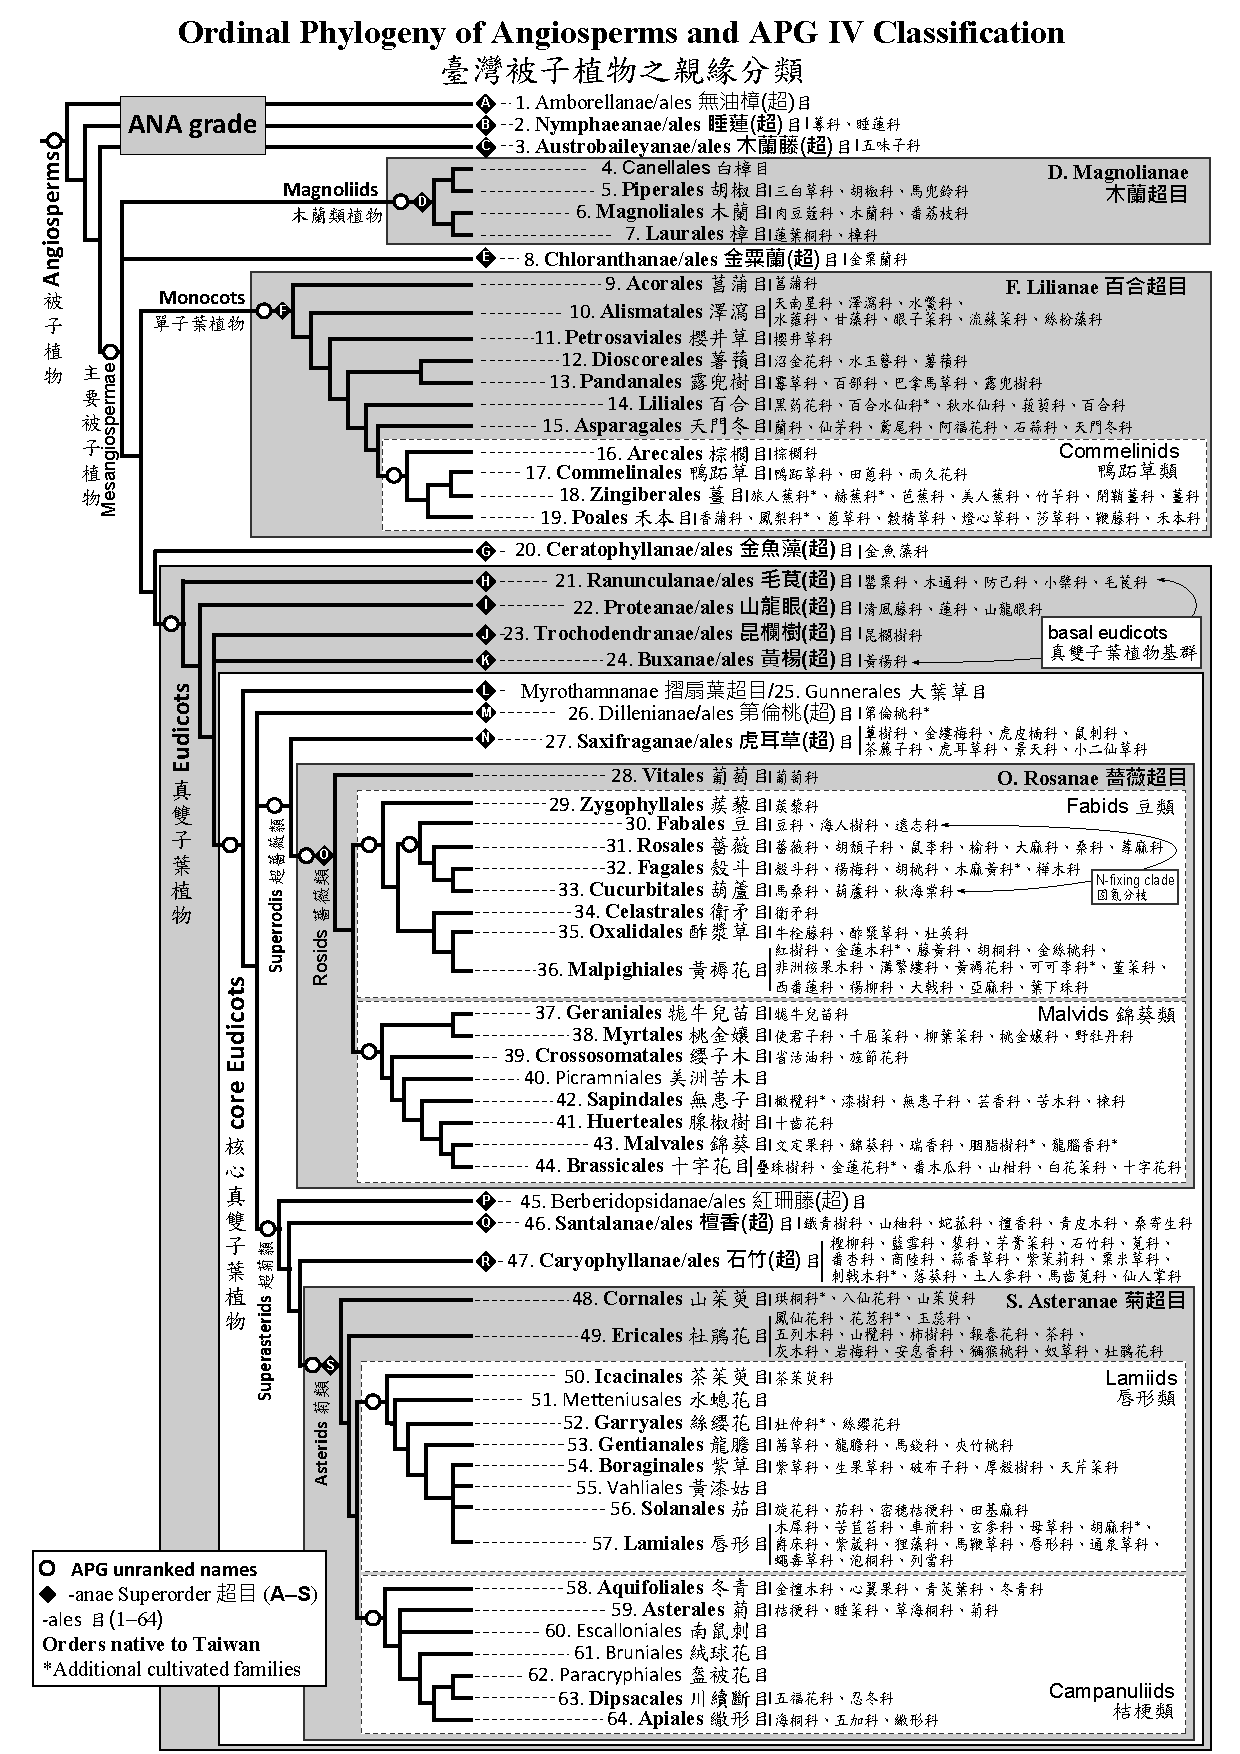
\includepdf{APGIV.pdf}
